%=================================================================
% This template is based on IMRT Latex template by Eric A. Mueller
%================================================================= 

\documentclass[10pt,twoside,a4paper]{report}

 \usepackage[mt,hs,english]{ethasl}   % New styles and commands
                                      % Options: 	bt/mt: Bachelorthesis/Masterthesis
                                      %						fs/hs: Fr�hlingssemester/Herbstsemester
                                      %						german/english: Deutsch/English

% \includeonly{}                      % Quick formatting
% \usepackage[draft]{graphicx}        % Quick formatting

 \usepackage{a4}                      % Paper size
 \usepackage[latin1]{inputenc}        % Keybord settings
 \usepackage{amsmath}                 % Additional math functionality
 \usepackage{amssymb}                 % Additional math functionality
 \usepackage{graphicx}                % EPS figures
 \usepackage[dvips]{epsfig}           % EPS figures
 \usepackage{float}                   % Placement of floating objects
 \usepackage{fancyhdr}                % Headings
 \usepackage{rotating}
 \usepackage{multirow}
 \usepackage{url}
 \usepackage{colortbl}
 \usepackage{ifpdf}
 

 \usepackage{hyperref}
 \usepackage{color}
 \definecolor{black}{rgb}{0,0,0}
 \definecolor{white}{rgb}{1,1,1}

 \definecolor{darkred}{rgb}{0.5,0,0}
 \definecolor{darkgreen}{rgb}{0,0.5,0}
 \definecolor{darkblue}{rgb}{0,0,0.5}

 \hypersetup{colorlinks
	,linkcolor=black
	,filecolor=black
	,urlcolor=black
	,citecolor=black
 }


 \ifpdf
	\usepackage[update]{epstopdf}
 \else
 \fi

% \usepackage{german}                  % German language
% \usepackage{ae}                      % German specials

%---------------------------------------------------------------------------

 \setlength{\parindent}{0em}                   % Disable parindent
 \rhead[\thepage]{\nouppercase{\rightmark}}    % Special headings
 \lhead[\nouppercase{\leftmark}]{\thepage}     % Special headings
 \cfoot{}                                      % Special headings

%---------------------------------------------------------------------------

 \title{Path Planning for Dynamic Maneuvers with Micro Aerial Vehicles}
 %\subtitle{bla bla bla}

 
 \studentA{Fabian Neusch\"{a}fer}
% \studentB{Student 2}
% \studentC{Student 3}
 
 

\supervisionA{Markus Achtelik}
\supervisionB{Michael Burri}
%\supervisionC{Supervisor C}
 

%===========================================================================
\begin{document}

%---------------------------------------------------------------------------
% Title page

 \maketitle
 \pagestyle{plain}
 \pagenumbering{roman}

%---------------------------------------------------------------------------
% Declaration of Originality

\pagestyle{empty}
% TODO Modify placeholders in declaration.tex
%---------------------------------------------------------------------------
% Declaration of Originality
%
% TODO Add title, student first/last name, supervisor first/last name.

\section*{Declaration of Originality}

\vspace{1cm}

I hereby declare that the written work I have submitted entitled

\vspace{0.5cm}

% TODO Add title
\textbf{Path Planning for Dynamic Maneuvers with Micro Aerial Vehicles}

\vspace{0.5cm}

is original work which I alone have authored and which is written in my own words.\footnote{Co-authored work: The signatures of all authors are required. Each signature attests to the originality of the entire piece of written work in its final form.}

\vspace{1cm}

\textbf{Author(s)}

\vspace{0.5cm}

\begin{tabular}{ p{5cm} p{5cm} }
% TODO Add student first/last name
  First name & Last name \\
\end{tabular}

\vspace{0.5cm}

\textbf{Supervising lecturer}

\vspace{0.5cm}

\begin{tabular}{ p{5cm} p{5cm} }
% TODO Add supervisor first/last name
  First name & Last name \\
\end{tabular}

\vspace{1cm}

With the signature I declare that I have been informed regarding normal academic citation rules and that I have read and understood the information on 'Citation etiquette' (\url{http://www.ethz.ch/students/exams/plagiarism_s_en.pdf}). The citation conventions usual to the discipline in question here have been respected.

\vspace{0.5cm}

The above written work may be tested electronically for plagiarism.

\vspace{4cm}

\begin{tabular}{ p{5cm} p{1cm} p{5cm} }
  \cline{1-1} \cline{3-3}
  Place and date & & Signature \\
\end{tabular}

%---------------------------------------------------------------------------



%---------------------------------------------------------------------------
% Preamble

 %---------------------------------------------------------------------------
% Preface

%\chapter*{Vorwort}

%Bla bla \dots

 %\cleardoublepage

%---------------------------------------------------------------------------
% Table of contents

 \setcounter{tocdepth}{2}
 \tableofcontents

 \cleardoublepage

%---------------------------------------------------------------------------
% Abstract

%\chapter*{Zusammenfassung}
% \addcontentsline{toc}{chapter}{Zusammenfassung}

%Bla bla \dots

% \cleardoublepage



\chapter*{Abstract}
 \addcontentsline{toc}{chapter}{Abstract}

The goal of this master thesis is to develop a numerical robust trajectory planning algorithm for dynamic multi-copter flights in dense environments. The trajectory generated by this algorithm is represented by polynomials which are jointly optimized. The cost function of the optimization consists of the total trajectory-time as well as the total quadratic snap (second derivation of the acceleration). The inclusion of the snap into the cost function guaranties a trajectory without abrupt or expensive control inputs. \newline

Furthermore, the process of exploring the state space using the Rapidly-Exploring Random Tree (RRT) algorithm is embedded into the numerical robust algorithm. The sampling points oft the RRT (or RRT*) algorithm are then used as the nodes in the polynomial optimization.


\newpage
% \cleardoublepage

%---------------------------------------------------------------------------
% Symbols

%\chapter*{Symbolverzeichnis}\label{chap:symbole}
% \addcontentsline{toc}{chapter}{Symbolverzeichnis}
\chapter*{Symbols}\label{chap:symbole}
 \addcontentsline{toc}{chapter}{Symbols}

%\section*{Symbole}
%\section*{Symbols}
%\begin{tabbing}
% \hspace*{3cm} \= \kill
%  $\phi, \theta, \psi$ 		\> roll, pitch and yaw angle \\[0.5ex] 							
% \end{tabbing}

%\section*{Indizes}
%\section*{Indices}
%\begin{tabbing}
% \hspace*{1.6cm}  \= \kill
% $x$ \> x axis \\[0.5ex]
% $y$ \> y axis \\[0.5ex]
% 
%\end{tabbing}

\section*{Terms and Definitions}
\begin{tabbing}
 \hspace*{1.6cm}  \= \kill
jerk \> Derivation of acceleration \\[0.5ex]
snap \> Derivation of jerk \\[0.5ex]
vertex \> Fixed sampling point of a polynomial trajectory \\[0.5ex]
\end{tabbing}

%\section*{Akronyme und Abk�rzungen}
\section*{Acronyms and Abbreviations}
\begin{tabbing}
 \hspace*{1.6cm}  \= \kill
 ETH \> Eidgen\"{o}ssische Technische Hochschule \\[0.5ex]
 QP \>  Quadratic Programming\\[0.5ex]
 UAV \> Unmanned Aerial Vehicle \\[0.5ex]
RRT \> Rapidly-Exploring Random Tree\\[0.5ex]
ROS \> Robot Operating System\\[0.5ex]
\end{tabbing}

 \cleardoublepage

%---------------------------------------------------------------------------


 \pagestyle{headings}                 % Default headings
 \pagestyle{fancy}                   % Special headings
 \pagenumbering{arabic}

%---------------------------------------------------------------------------
% Chapters

 
\chapter{Introduction}\label{sec:introduction}

\section{State of the Art}\label{sec:state}

A lot of research has been performed in the field of Unmanned Aerial Vehicles (UAV) in the last years leading to a strong improvement in trajectory planning \cite{he} as well as in control (\cite{colling}, \cite{hehn}).  Another field of research is machine learning \cite{lup} which is suitable to enhance the performance of aerobatic maneuvers but seems to have a downside regarding motion planning and trajectory generation in dense environments. \newline

Speaking of trajectory planning, there are two different strategies which are pursued. On the one hand, the geometric and the temporal planning are decoupled  \cite{bou}, on the other hand geometric and temporal information are coupled and the trajectory is the result of a minimization problem. For the coupled problem one can make use of the differential flatness of a quadrocopter to derive constraint on the trajectory. A cost function which could be the total trajectory-time \cite{hehn} or the total snap \cite{mellinger} can be formulated. \newline


%Then formulate a cost-function which could be the trajectory-time \cite{hehn} or the total snap \cite{mellinger} (second %derivation of acceleration). \newline

Another aspect of planning is exploring the state space in the first place. A strong tool to do so are incremental search techniques as for instance the A* \cite{lik} or the RRT* algorithm \cite{richter}. The sampling points of the solution of the incremental search can then be used as the nodes for the polynomial optimization.

\section{Quadratic Programming}\label{sec:quadratic}

As mentioned above, the snap can be used as the cost function in trajectory optimization. Regarding snap minimization, Quadratic Programming (QP) is a powerful tool.

\subsection{Constrained Quadratic Programming}

QP is a special case of an optimization problem in which a quadratic function $f(x)$ is optimized with respect to its optimization variables (which are represented with the vector $x$ in equation \ref{equ:quadratic})

\begin{equation}
 f(x)  = \frac{1}{2} \cdot x^T Q x + c^T x 
\label{equ:quadratic}
\end{equation}

The optimization can be performed under linear constraints on the optimization variables. The linear constraints can be divided in two groups. \newline

 For one thing there are the inequality constraints

\begin{equation}
A  x \leq b
\label{equ:inequalityConstraintsQP}
\end{equation}

where the vector $b$ contains the inequality constraints. For another thing there are the equality constraints

\begin{equation}
E  x = d
\end{equation}

where the vector $d$ contains the equality constraints. In case there are only equality constraints, the solution to the QP is given by the linear system in equation \ref{equ:equality} :



% Whereas a distinction between equality($ E\mathbf{x} = \mathbf d $) and inequality constraints ($ A\mathbf{x} \leq \mathbf b $) has to be made. 
%In case there are only equality constraints, the solution to the QP is given by the linear system in equation \ref{equ:equality} :


\begin{equation}
\begin{bmatrix}
   Q & E^T \\
   E & 0
\end{bmatrix} 
\cdot
\begin{bmatrix}
   \mathbf x \\
   \lambda
\end{bmatrix}
= 
\begin{bmatrix}
   -\mathbf c \\
   \mathbf d
\end{bmatrix}
\label{equ:equality}
\end{equation}


where $\lambda$ is a set of Lagrange multipliers and $c$ is the linear term of the cost function in equation \ref{equ:quadratic}. \newline

The constrained QP gets ill-conditioned for a large number of optimization variables which lead to large matrices. The performance of the constraint QP deteriorates even more if the matrices are sparse. This particular case often appears in polynomial optimization for high order polynomials where some polynomial coefficients are close to zero. \newline

To reduce the number of optimization variables, and therefore the size of the matrices, the constrained QP with equality constraints can be converted into a numerical robust unconstrained QP. This is one of the goals of this master thesis.

\subsection{Unconstrained Quadratic Programming}

For the unconstrained QP the equality constraints $E \mathbf{x} = \mathbf{d}$ resp. $\mathbf{x} = E^{-1} \mathbf{d}$ are embedded into the quadratic cost function from equation \ref{equ:quadratic} resulting in equation \ref{equ:quadratic_unconstrained}:

\begin{equation}
 f(d)  = \frac{1}{2} \cdot d^T  E^{-T}  Q  E^{-1}  d + c^T  E^{-1} d
\label{equ:quadratic_unconstrained}
\end{equation}

Since the vector $x$ is replaced by $E^{-1} d$ and $E$ is a constant matrix, the new optimization variables are now stored in the vector $d$. \newline
 
%Referring to polynomial trajectory optimization, the vector $x$ containing the polynomial coefficients is now replaced by the vector $d$ containing the endpoint derivatives and the mapping matrix $E$. In other words, the polynomial coefficients are no longer the optimization variables but the free endpoint derivatives are optimized. Furthermore the polynomial trajectory optimization does not have a linear term $c^T \mathbf{x}$. Hence Equation \ref{equ:quadratic_unconstrained} can be simplified to:  

If the cost function defined in equation \ref{equ:quadratic} does not have a linear term, i.e. the vector $c$ is equal to zero, equation \ref{equ:quadratic_unconstrained} can be simplified to:

\begin{equation}
 f(d)  = \frac{1}{2} \cdot d^T  E^{-T}  Q  E^{-1}  d 
\label{equ:quadratic_simple}
\end{equation}

If we are not interested  in the cost itself but only in the optimization variables stored in $d$, the constant multiplier $1/2$ can be dropped:

\begin{equation}
 f(d)  = d^T  E^{-T}  Q  E^{-1}  d 
\label{equ:quadratic_short}
\end{equation}

The theoretical derived equation \ref{equ:quadratic_short} will be compared to to multidimensional cost function in equation \ref{equ:uncon_cost}. Equation \ref{equ:uncon_cost} establishes a connection between the numerical advantages of a unconstrained QP and the polynomial coefficients representing a trajectory.













 \cleardoublepage
 
\chapter{Einige wichtige Hinweise zum Arbeiten mit \LaTeX\ }\label{sec:latexumg}

Nachfolgend wird die Codierung einiger oft verwendeten Elemente
kurz beschrieben. Das Einbinden von Bildern ist in \LaTeX\ nicht
ganz unproblematisch und h�ngt auch stark vom verwendeten Compiler
ab. Typisches Format f�r Bilder in \LaTeX\ ist
EPS\footnote{Encapsulated Postscript}.


\section{Gliederungen}\label{sec:gliederung}

Ein Text kann mit den Befehlen \texttt{\textbackslash
chapter\{.\}}, \texttt{\textbackslash section\{.\}},
\texttt{\textbackslash subsection\{.\}} und \texttt{\textbackslash
subsubsection\{.\}} gegliedert werden.


\section{Referenzen und Verweise}\label{sec:refverw}

Literaturreferenzen werden mit dem Befehl \texttt{\textbackslash
cite\{.\}} erzeugt. Ein Beispiel: \cite{comfilt}.

Zur Erzeugung von Fussnoten wird der Befehl \texttt{\textbackslash
footnote\{.\}} verwendet. Auch hier ein Beispiel\footnote{Bla
bla.}.

Querverweise im Text werden mit \texttt{\textbackslash label\{.\}}
verankert und mit \texttt{\textbackslash ref\{.\}} erzeugt.
Beispiel einer Referenz auf das zweite Kapitel:
Kapitel~\ref{sec:latexumg}.


\section{Aufz�hlungen}\label{sec:aufz}

Folgendes Beispiel einer Aufz�hlung ohne Numerierung,
\begin{itemize}
  \item Punkt 1
  \item Punkt 2
\end{itemize}
wurde erzeugt mit:
\begin{verbatim}
\begin{itemize}
  \item Punkt 1
  \item Punkt 2
\end{itemize}
\end{verbatim}

Folgendes Beispiel einer Aufz�hlung mit Numerierung,
\begin{enumerate}
  \item Punkt 1
  \item Punkt 2
\end{enumerate}
wurde erzeugt mit:
\begin{verbatim}
\begin{enumerate}
  \item Punkt 1
  \item Punkt 2
\end{enumerate}
\end{verbatim}

Folgendes Beispiel einer Auflistung,
\begin{description}
  \item[P1] Punkt 1
  \item[P2] Punkt 2
\end{description}
wurde erzeugt mit:
\begin{verbatim}
\begin{description}
  \item[P1] Punkt 1
  \item[P2] Punkt 2
\end{description}
\end{verbatim}


\section{Erstellen einer Tabelle}\label{sec:tabellen}

Ein Beispiel einer Tabelle:
\begin{table}[h]
\begin{center}
 \caption{Daten der Fahrzyklen ECE, EUDC, NEFZ.}\vspace{1ex}
 \label{tab:tabnefz}
 \begin{tabular}{ll|ccc}
 \hline
 Kennzahl & Einheit & ECE & EUDC & NEFZ \\ \hline \hline
 Dauer & s & 780 & 400 & 1180 \\
 Distanz & km & 4.052 & 6.955 & 11.007 \\
 Durchschnittsgeschwindigkeit & km/h & 18.7 &  62.6 & 33.6 \\
 Leerlaufanteil & \% & 36 & 10 & 27 \\
 \hline
 \end{tabular}
\end{center}
\end{table}

Die Tabelle wurde erzeugt mit:
\begin{verbatim}
\begin{table}[h]
\begin{center}
 \caption{Daten der Fahrzyklen ECE, EUDC, NEFZ.}\vspace{1ex}
 \label{tab:tabnefz}
 \begin{tabular}{ll|ccc}
 \hline
 Kennzahl & Einheit & ECE & EUDC & NEFZ \\ \hline \hline
 Dauer & s & 780 & 400 & 1180 \\
 Distanz & km & 4.052 & 6.955 & 11.007 \\
 Durchschnittsgeschwindigkeit & km/h & 18.7 &  62.6 & 33.6 \\
 Leerlaufanteil & \% & 36 & 10 & 27 \\
 \hline
 \end{tabular}
\end{center}
\end{table}
\end{verbatim}


\section{Einbinden einer EPS-Graphik}\label{sec:epsgraph}

Das Einbinden von Graphiken kann wie folgt bewerkstelligt werden:
\begin{verbatim}
\begin{figure}[h]
   \centering
   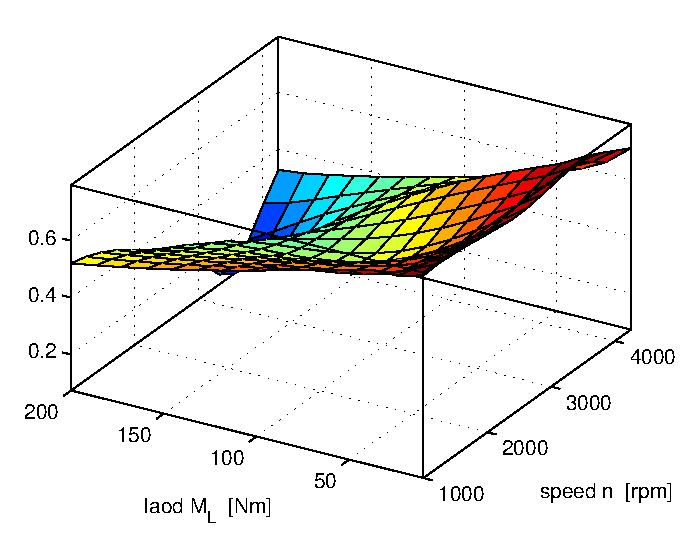
\includegraphics[width=0.75\textwidth]{pics/k_surf.eps}
   \caption{Ein Bild.}
   \label{pics:k_surf}
\end{figure}
\end{verbatim}

\begin{figure}[h]
   \centering
   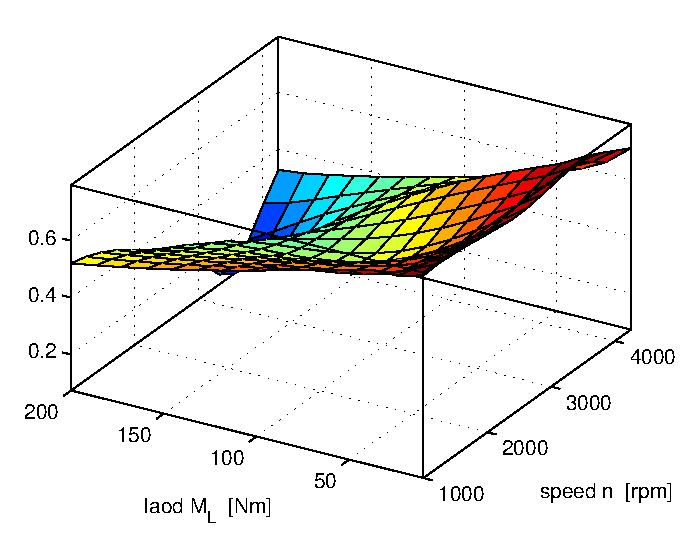
\includegraphics[width=0.75\textwidth]{pics/k_surf.eps}
   \caption{Ein Bild.}
   \label{pics:k_surf}
\end{figure}

oder bei zwei Bildern nebeneinander mit:
\begin{verbatim}
\begin{figure}[h]
  \begin{minipage}[t]{0.48\textwidth}
    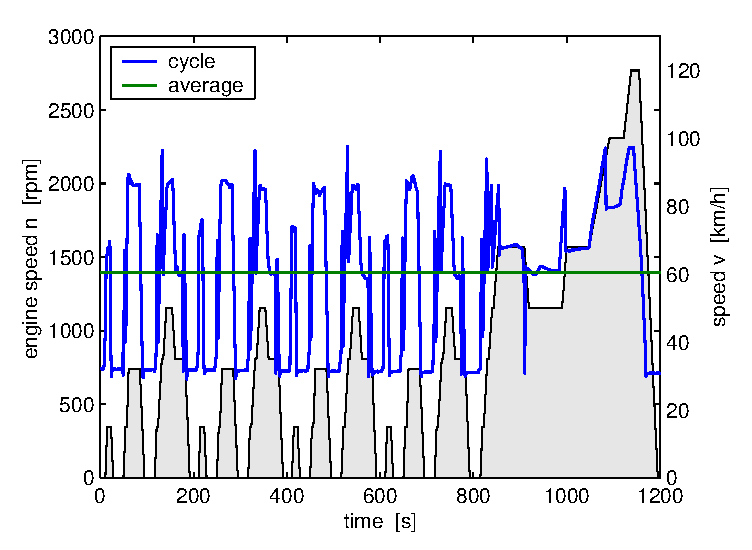
\includegraphics[width = \textwidth]{pics/cycle_we.eps}
  \end{minipage}
  \hfill
  \begin{minipage}[t]{0.48\textwidth}
    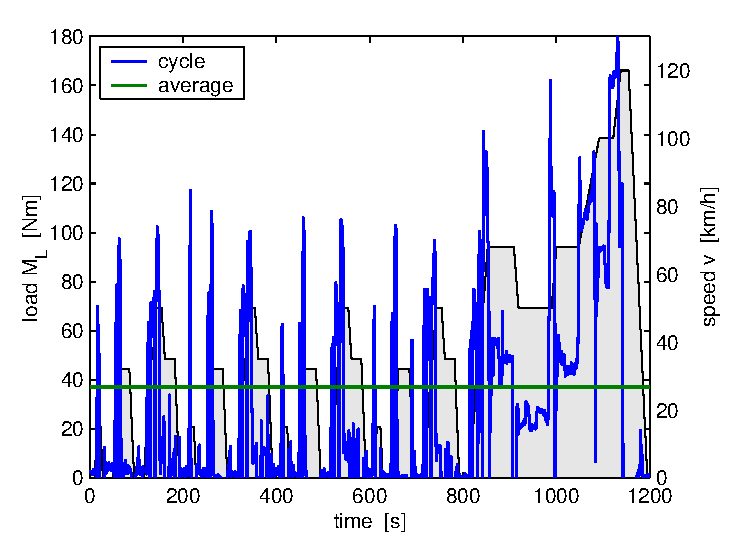
\includegraphics[width = \textwidth]{pics/cycle_ml.eps}
  \end{minipage}
  \caption{Zwei Bilder nebeneinander.}
  \label{pics:cycle}
\end{figure}
\end{verbatim}

\begin{figure}[h]
  \begin{minipage}[t]{0.48\textwidth}
    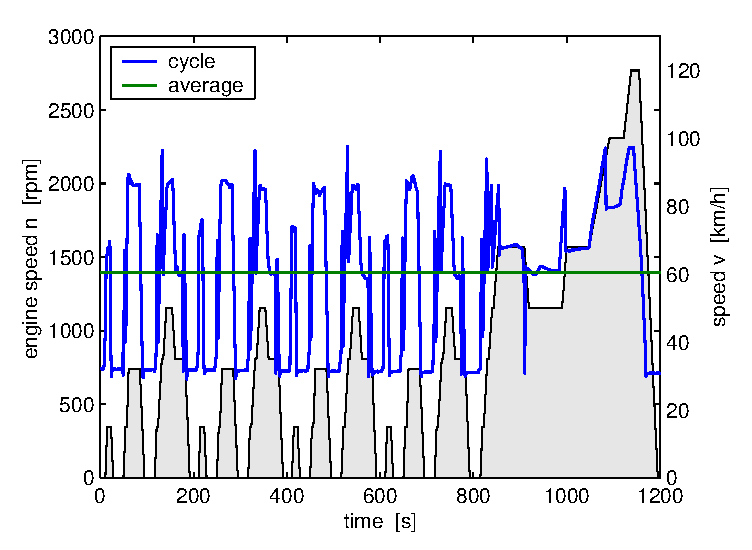
\includegraphics[width = \textwidth]{pics/cycle_we.eps}
  \end{minipage}
  \hfill
  \begin{minipage}[t]{0.48\textwidth}
    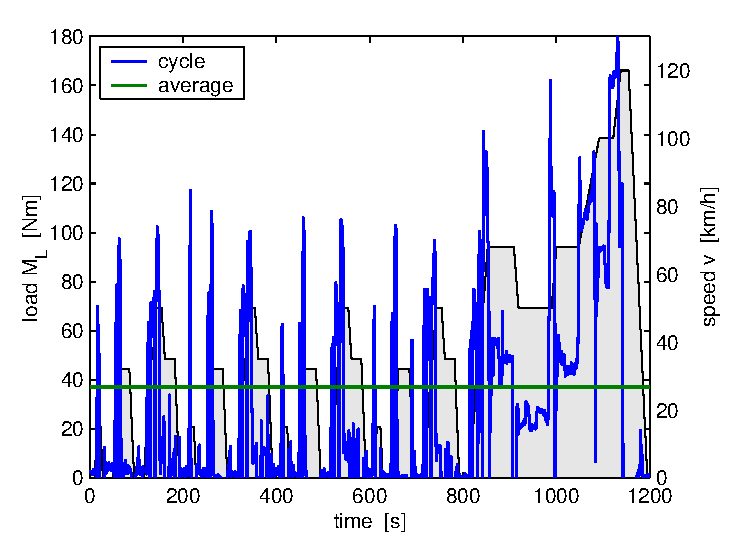
\includegraphics[width = \textwidth]{pics/cycle_ml.eps}
  \end{minipage}
  \caption{Zwei Bilder nebeneinander.}
  \label{pics:cycle}
\end{figure}

Bemerkung: Ersetzt man den Positionierungsparameter \texttt{h}
durch \texttt{H}, so wird das Gleiten der Abbildung verhindert.


\section{Mathematische Formeln}\label{sec:math}

Einfache mathematische Formeln werden mit der equation-Umgebung
erzeugt:
\begin{equation}
 p_{me0f}(T_e,\omega_e) \ = \ k_1(T_e) \cdot (k_2+k_3 S^2
 \omega_e^2) \cdot \Pi_{max} \cdot \sqrt{\frac{k_4}{B}} \, .
\end{equation}

Der Code dazu lautet:
\begin{verbatim}
\begin{equation}
 p_{me0f}(T_e,\omega_e) \ = \ k_1(T_e) \cdot (k_2+k_3 S^2
 \omega_e^2) \cdot \Pi_{max} \cdot \sqrt{\frac{k_4}{B}} \, .
\end{equation}
\end{verbatim}

Mathematische Ausdr�cke im Text werden mit \$formel\$ erzeugt (zB:
$a^2+b^2=c^2$).


\section{Weitere n�tzliche Befehle}\label{sec:div}

Hervorhebungen im Text sehen so aus: \emph{hervorgehoben}. Erzeugt
werden sie mit dem \texttt{\textbackslash epmh\{.\}} Befehl.

 \cleardoublepage
% \include{}
% \cleardoublepage
% \include{}
% \cleardoublepage
% ...
%
%---------------------------------------------------------------------------
% Appendix

 \appendix
 
\chapter{Irgendwas}\label{sec:irgendwas}

Bla bla \dots

 \cleardoublepage

%
%\chapter{Nochmals irgendwas}\label{sec:nochirgendwas}
%
%Bla bla \dots
%
% \cleardoublepage

%
%---------------------------------------------------------------------------
% Literature

 
\begin{thebibliography}{99}
%\addcontentsline{toc}{chapter}{Literaturverzeichnis}
\addcontentsline{toc}{chapter}{Bibliography}



\bibitem {he} {\sc R. He, A. Bachrach, M. Achtelik, A. Geramifard, D. Gurdan, S. Prentice,
J. Stumpf, and N. Roy}: 
{\it On the design and use of a micro air
vehicle to track and avoid adversaries}. The Int. Journal of Robotics
Research, vol. 29, pp. 529-546, 2010.


\bibitem {colling} {\sc D. Colling, O. A.~Yakimenko, J. F.~Whidborne, and A. K.~Cooke}:
{\it A prototype of an autonomous controller for a quadrotor UAV}. In
Proceedings of the European Control Conference, Kos, Greece, 2007,
pp. 1-8.


\bibitem {hehn} {\sc M. Hehn and R. D'Andrea }:
{\it Quadrocopter trajectory generation and control}. In
International Federation of Automatic Control (IFAC), World Congress 2011, 2011.


\bibitem {lup} {\sc S. Lupashin, A. Schollig, M. Sherback, and R. D'Andrea}:
 {\it A simple learning strategy for high-speed quadrocopter multi-flips}.
In Proc. of the IEEE Int. Conf. on Robotics and Automation, Anchorage, AK,
May 2010, pp. 1642-1648.


\bibitem {bou} {\sc Y. Bouktir, M. Haddad, and T. Chettibi}:
{\it Trajectory Planning for a
Quadrotor Helicopter}. In Mediterranean Conference on Control and
Automation, Jun. 2008, pp. 1258-1263


\bibitem {mellinger} {\sc D. Mellinger and V. Kumar}: 
{\it Minimum snap trajectory generation and
control for quadrotors}. In International Conference on Robotics and
Automation, 2011, pp. 2520-2525.

\bibitem {lik} {\sc M. Likhachev, G. Gordon and S. Thrun}: 
{\it  ARA*: Anytime A* with Provable Bounds on Sub-Optimality }.
Advances in Neural Information
Processing Systems, vol. 16, 2003

\bibitem {richter} {\sc C. Richter,  A. Bry, and N, Roy}: 
{\it  Polynomial Trajectory Planning
for Quadrotor Flight}.
In International Conference on Robotics and
Automation, 2013.



\end{thebibliography}


%---------------------------------------------------------------------------

\end{document}
%===========================================================================
